%% ============================================================
%%  MEMORIA TÉCNICA — cv-lit
%%  Sistema de Monitorización Automática de Línea de Costa
%%  Guardamar del Segura · Universidad de Alicante · 2026
%% ============================================================
\documentclass[12pt,a4paper,spanish]{report}

% -- Codificación y tipografía --------------------------------
\usepackage[T1]{fontenc}
\usepackage[utf8]{inputenc}
\usepackage{babel}
\usepackage{lmodern}
\usepackage{microtype}

% -- Geometría ------------------------------------------------
\usepackage[
  top=2.5cm, bottom=2.5cm,
  left=3.0cm, right=2.5cm,
  headheight=15pt
]{geometry}

% -- Color y gráficos -----------------------------------------
\usepackage[dvipsnames,svgnames,table]{xcolor}
\usepackage{graphicx}
\usepackage{float}
\usepackage{wrapfig}
\usepackage{subcaption}

% -- Tablas ---------------------------------------------------
\usepackage{booktabs}
\usepackage{longtable}
\usepackage{multirow}
\usepackage{array}
\usepackage{tabularx}
\newcolumntype{L}[1]{>{\raggedright\arraybackslash}p{#1}}
\newcolumntype{C}[1]{>{\centering\arraybackslash}p{#1}}

% -- Código fuente --------------------------------------------
\usepackage{listings}
\usepackage{minted}
\setminted{
  fontsize=\footnotesize,
  linenos=true,
  breaklines=true,
  frame=lines,
  framesep=6pt,
  baselinestretch=1.1,
  bgcolor=gray!5
}
\lstset{
  basicstyle=\ttfamily\footnotesize,
  breaklines=true,
  frame=single,
  backgroundcolor=\color{gray!8},
  keywordstyle=\color{NavyBlue}\bfseries,
  commentstyle=\color{OliveGreen},
  stringstyle=\color{BrickRed},
  numberstyle=\tiny\color{gray},
  numbers=left,
  numbersep=6pt
}

% -- Matemáticas ----------------------------------------------
\usepackage{amsmath,amssymb}

% -- Cabeceras y pies -----------------------------------------
\usepackage{fancyhdr}
\pagestyle{fancy}
\fancyhf{}
\fancyhead[L]{\small\textit{cv-lit — Sistema de Monitorización Costera}}
\fancyhead[R]{\small\textit{\leftmark}}
\fancyfoot[C]{\thepage}
\renewcommand{\headrulewidth}{0.4pt}

% -- Hiperenlaces ---------------------------------------------
\usepackage[
  colorlinks=true,
  linkcolor=NavyBlue,
  citecolor=OliveGreen,
  urlcolor=Teal,
  pdftitle={Memoria Técnica cv-lit},
  pdfauthor={Tech4D Lab — Universidad de Alicante}
]{hyperref}

% -- Cajas de información -------------------------------------
\usepackage{tcolorbox}
\tcbuselibrary{skins,breakable,listings}
\newtcolorbox{infobox}[1][]{
  colback=SkyBlue!10, colframe=NavyBlue!70,
  fonttitle=\bfseries, title=#1,
  breakable, left=6pt, right=6pt, top=4pt, bottom=4pt
}
\newtcolorbox{warnbox}[1][]{
  colback=Goldenrod!12, colframe=Goldenrod!80,
  fonttitle=\bfseries, title=#1,
  breakable, left=6pt, right=6pt, top=4pt, bottom=4pt
}
\newtcolorbox{codebox}[1][]{
  colback=gray!6, colframe=gray!40,
  fonttitle=\bfseries\ttfamily, title=#1,
  breakable, left=4pt, right=4pt, top=2pt, bottom=2pt
}

% -- Diagrama de flujo (TikZ) ---------------------------------
\usepackage{tikz}
\usetikzlibrary{shapes.geometric, arrows.meta, positioning, fit, backgrounds, shadows}
\tikzset{
  block/.style={
    rectangle, rounded corners=4pt, minimum width=4.5cm, minimum height=1cm,
    text centered, draw=NavyBlue!70, fill=NavyBlue!8,
    font=\small\sffamily, drop shadow
  },
  decision/.style={
    diamond, aspect=2.5, minimum width=3.5cm, minimum height=1cm,
    text centered, draw=BrickRed!70, fill=BrickRed!8,
    font=\small\sffamily
  },
  arrow/.style={-{Stealth[length=5pt]}, thick, color=gray!70},
  label/.style={font=\tiny\sffamily, color=gray!80}
}

% -- Misc -----------------------------------------------------
\usepackage{enumitem}
\usepackage{setspace}
\usepackage{titlesec}
\usepackage{pdflscape}
\usepackage{afterpage}
\usepackage{parskip}
\setlength{\parskip}{6pt}

\titleformat{\chapter}[display]
  {\normalfont\huge\bfseries\color{NavyBlue}}
  {\chaptertitlename\ \thechapter}{20pt}{\Huge}
\titlespacing*{\chapter}{0pt}{30pt}{40pt}

\titleformat{\section}
  {\normalfont\Large\bfseries\color{NavyBlue!80}}
  {\thesection}{1em}{}
\titleformat{\subsection}
  {\normalfont\large\bfseries\color{NavyBlue!60}}
  {\thesubsection}{1em}{}

% -- Metadatos ------------------------------------------------
\title{%
  \vspace{-1.5cm}
  \textbf{\Huge Memoria Técnica}\\[0.4cm]
  {\Large\textcolor{NavyBlue}{cv-lit}}\\[0.2cm]
  {\large Sistema de Monitorización Automática}\\
  {\large de Línea de Costa}\\[0.6cm]
  \rule{\linewidth}{1pt}\\[0.4cm]
  {\normalsize Guardamar del Segura · Alicante · España}
}
\author{
  \textbf{Tech4D Lab}\\
  Universidad de Alicante\\
  \texttt{nickhernd}
}
\date{Junio 2026}

%% ============================================================
\begin{document}
%% ============================================================

\maketitle
\thispagestyle{empty}

\begin{abstract}
\noindent
\textbf{cv-lit} es un sistema software de monitorización automática de línea de costa mediante
visión por computador, desarrollado para el Ayuntamiento de Guardamar del Segura
en colaboración con el Instituto de Ecología Litoral (IEL) y la Universidad de Alicante.

El sistema procesa imágenes oblicuas de \textbf{6 cámaras fijas Obscape} instaladas a lo largo del
frente litoral (tramo norte--sur $\approx$ 3,5~km), extrayendo automáticamente la línea de costa
y proyectándola a coordenadas geográficas UTM EPSG:25830 (ETRS89 / UTM zona 30N).

Esta memoria recoge la arquitectura completa del sistema, los algoritmos de procesamiento
de imagen (SIFT, RANSAC, SAM), el módulo de alineación masiva no-destructiva diseñado en la
iteración de junio de 2026, la interfaz web de validación por lotes, los resultados de
calibración geométrica obtenidos para las seis cámaras, y la documentación operacional
completa para el despliegue y mantenimiento del sistema.
\end{abstract}

\tableofcontents
\listoffigures
\listoftables

% ==============================================================
\chapter{Descripción del Proyecto}
\label{ch:overview}
% ==============================================================

\section{Contexto y motivación}

La playa de Guardamar del Segura es un espacio de alto valor ecológico y turístico sujeto a
procesos de erosión y acreción que requieren seguimiento sistemático. La medición manual de la
línea de costa mediante levantamientos GNSS es costosa, puntual y no escala para cubrir todo el
frente litoral con frecuencia horaria.

El proyecto \textbf{cv-lit} surge para automatizar esta medición aprovechando la infraestructura
de cámaras fijas ya desplegada por el servicio de vigilancia de la playa, convirtiendo cada
fotografía en un dato georreferenciado de la posición de la interfaz arena--mar.

\section{Partes implicadas}

\begin{table}[H]
\centering
\caption{Actores del proyecto}
\label{tab:actors}
\begin{tabular}{L{4cm} L{9cm}}
\toprule
\textbf{Rol} & \textbf{Entidad} \\
\midrule
Cliente & Ayuntamiento de Guardamar del Segura \\
Datos GNSS (GCPs) & Instituto de Ecología Litoral (IEL) \\
Desarrollo & 1 ingeniero a tiempo parcial (Tech4D Lab, UA) \\
Supervisión & Universidad de Alicante \\
Duración & 6 meses (enero -- junio 2026) \\
\bottomrule
\end{tabular}
\end{table}

\section{Objetivos del sistema}

El producto final es un \textbf{GeoJSON proyectado en EPSG:25830} con los siguientes atributos
obligatorios por cada detección:

\begin{table}[H]
\centering
\caption{Atributos del GeoJSON de salida}
\label{tab:geojson-fields}
\begin{tabular}{L{3.5cm} L{3.5cm} L{5.5cm}}
\toprule
\textbf{Campo} & \textbf{Tipo} & \textbf{Descripción} \\
\midrule
\texttt{ID\_Camara}    & Integer (1--6) & Identificador de cámara origen \\
\texttt{Timestamp}     & ISO 8601 UTC   & Fecha y hora de captura \\
\texttt{Confianza\_IA} & Float (0--1)   & Score de confianza del modelo SAM \\
\texttt{Area\_Seca\_m2}& Float          & Superficie de playa seca (m²) \\
\bottomrule
\end{tabular}
\end{table}

\section{Restricciones no negociables}

\begin{itemize}[leftmargin=1.5em]
  \item Toda implementación \textbf{debe} producir GeoJSON en \textbf{EPSG:25830}.
  \item Fase horaria prioritaria: \textbf{12:00h solar local}.
  \item Modelo de segmentación: \textbf{SAM} (Segment Anything Model, Meta AI).
  \item Cada cámara tiene su propio perfil de calibración \textit{independiente}.
  \item Criterio de aceptación de precisión: \textbf{RMSE~$<$~1,5~m} en condiciones estándar.
\end{itemize}

\section{Entregables}

\begin{enumerate}[leftmargin=1.5em]
  \item Aplicación ejecutable configurada y documentada (esta memoria).
  \item Perfiles de calibración por cámara (6~ficheros \texttt{.npy} / \texttt{.json}).
  \item Interfaz web de operación y validación por lotes.
  \item Informe de validación con métricas RMSE y MAE.
\end{enumerate}

% ==============================================================
\chapter{Infraestructura de Cámaras}
\label{ch:cameras}
% ==============================================================

\section{Sistema Obscape}

Las seis cámaras están gestionadas por la plataforma Obscape y se acceden via API REST
autenticada. La tabla~\ref{tab:cameras} lista los parámetros de registro de cada estación.

\begin{table}[H]
\centering
\caption{Estaciones Obscape en Guardamar del Segura}
\label{tab:cameras}
\resizebox{\textwidth}{!}{%
\begin{tabular}{C{1.2cm} C{1.5cm} C{2.3cm} C{2.8cm} C{2.8cm} C{2cm}}
\toprule
\textbf{Cámara} & \textbf{Station} & \textbf{Referencia} & \textbf{Latitud (°N)} & \textbf{Longitud (°E)} & \textbf{Última act.} \\
\midrule
CAM~1 & 8213 & PTM61471 & 38.110327 & $-$0.643027 & 20-05-2026 \\
CAM~2 & 8214 & PTM61474 & 38.096291 & $-$0.645725 & 20-05-2026 \\
CAM~3 & 8212 & PTM61473 & 38.087348 & $-$0.646994 & 20-05-2026 \\
CAM~4 & 8211 & PTM61475 & 38.087385 & $-$0.647078 & 20-05-2026 \\
CAM~5 & 8209 & PTM61472 & 38.076774 & $-$0.648117 & 20-05-2026 \\
CAM~6 & 8210 & PTM61470 & 38.076796 & $-$0.648114 & 20-05-2026 \\
\bottomrule
\end{tabular}}
\end{table}

\begin{warnbox}[Nota geográfica]
CAM~3 y CAM~4 son casi coincidentes ($\Delta \approx 8$~m) y cubren el mismo tramo desde
ángulos ligeramente distintos. Lo mismo ocurre con CAM~5 y CAM~6. Esto permite comparación
cruzada de la línea detectada para validación interna.
\end{warnbox}

\section{Distribución geográfica}

Las cámaras se distribuyen de norte a sur a lo largo de $\approx 3{,}5$~km de frente litoral.
La cobertura solapada garantiza continuidad en la extracción de línea de costa sin lagunas.

\section{Descarga automática de imágenes}

El módulo \texttt{acces\_api/scheduled\_download.py} implementa una \textbf{ventana deslizante de
14 días} que garantiza recuperación automática ante fallos puntuales de descarga:

\begin{codebox}[Descarga estándar]
\begin{minted}{bash}
# Últimas 2 semanas, hora solar 12:00 (por defecto)
python3 acces_api/scheduled_download.py

# Personalizar ventana y hora
python3 acces_api/scheduled_download.py --days 30 --hour 15

# Descarga masiva histórica (todas las horas)
python3 acces_api/scheduled_download.py --days 90 --hour all
\end{minted}
\end{codebox}

El sistema evita duplicados comprobando la existencia del fichero antes de descargar y utiliza
un nombre determinista: \texttt{UNIX\_YYYYMMDD\_HHMMSS\_REF.jpg}.

\subsection{Automatización con Cron}

Para descarga diaria autónoma:

\begin{codebox}[/etc/cron.d/cvlit-download]
\begin{minted}{text}
# Descarga diaria a las 13:00h (12h solar + margen de publicación API)
0 13 * * * cd /home/nickhernd/Desktop/cv-lit && \
  python3 acces_api/scheduled_download.py >> data/logs/cron.log 2>&1
\end{minted}
\end{codebox}

% ==============================================================
\chapter{Arquitectura del Sistema}
\label{ch:architecture}
% ==============================================================

\section{Stack tecnológico}

\begin{table}[H]
\centering
\caption{Dependencias principales}
\label{tab:stack}
\begin{tabular}{L{4cm} L{3.5cm} L{5cm}}
\toprule
\textbf{Componente} & \textbf{Versión} & \textbf{Rol} \\
\midrule
Python        & 3.11         & Runtime principal \\
FastAPI       & $\geq$ 0.110 & API REST backend \\
OpenCV        & 4.x          & Procesamiento de imagen \\
NumPy/SciPy   & --           & Álgebra matricial \\
SAM (Meta AI) & --           & Segmentación semántica \\
PyTorch       & $\geq$ 2.0   & Backend SAM \\
GDAL/pyproj   & --           & Transformaciones EPSG \\
Vue 3 + Vite  & --           & Interfaz web \\
Tailwind CSS  & 3.x          & Estilos \\
\bottomrule
\end{tabular}
\end{table}

\section{Estructura de directorios}

\begin{codebox}[Árbol del repositorio]
\begin{minted}{text}
cv-lit/
+-- acces_api/              # Módulo Obscape API
|   +-- obscape_api.py      # Cliente REST
|   +-- scheduled_download.py
+-- backend/                # Servidor FastAPI
|   +-- main.py             # App principal + routers
|   +-- batch_alignment.py  # Pipeline de alineación masiva  [NUEVO]
|   +-- config.py           # Constantes globales
|   +-- routers/
|       +-- alignment.py    # Endpoints unitarios de alineación
+-- calibration/            # Perfiles y máscaras por cámara
|   +-- cam_N_H.npy         # Matriz H 3×3 en float64
|   +-- cam_N_profile.json  # Metadatos, RMSE, fecha
|   +-- roi_config.json     # ROIs por cámara
|   +-- alignment_masks.json# Zonas SIFT estables  [NUEVO]
|   +-- diagnostics/        # Imágenes de diagnóstico
+-- data/                   # Imágenes y resultados (excl. Git)
|   +-- CAM_N/
|   |   +-- images/         # Originales
|   |   +-- aligned/        # Salida del commit de batch
|   +-- logs/
+-- docs/                   # Documentación técnica
|   +-- memoria.tex         # Esta memoria  [NUEVO]
|   +-- reports/
+-- frontend/               # Interfaz Vue 3
|   +-- src/components/
|       +-- App.vue
|       +-- Calibration.vue
|       +-- BatchAlignment.vue  [NUEVO]
+-- homography/
|   +-- align_images.py     # CLI standalone de alineación
+-- proces_images/          # Algoritmos de procesamiento
|   +-- calibration_tool.py
|   +-- extract_coastline.py
|   +-- segmentation_sam.py
|   +-- recalibrate.py
+-- scripts/                # Herramientas de operación
+-- tests/
\end{minted}
\end{codebox}

\section{Pipeline de procesamiento}

La figura~\ref{fig:pipeline} muestra el grafo completo de procesamiento desde la adquisición
hasta la exportación del GeoJSON georreferenciado.

\begin{figure}[H]
\centering
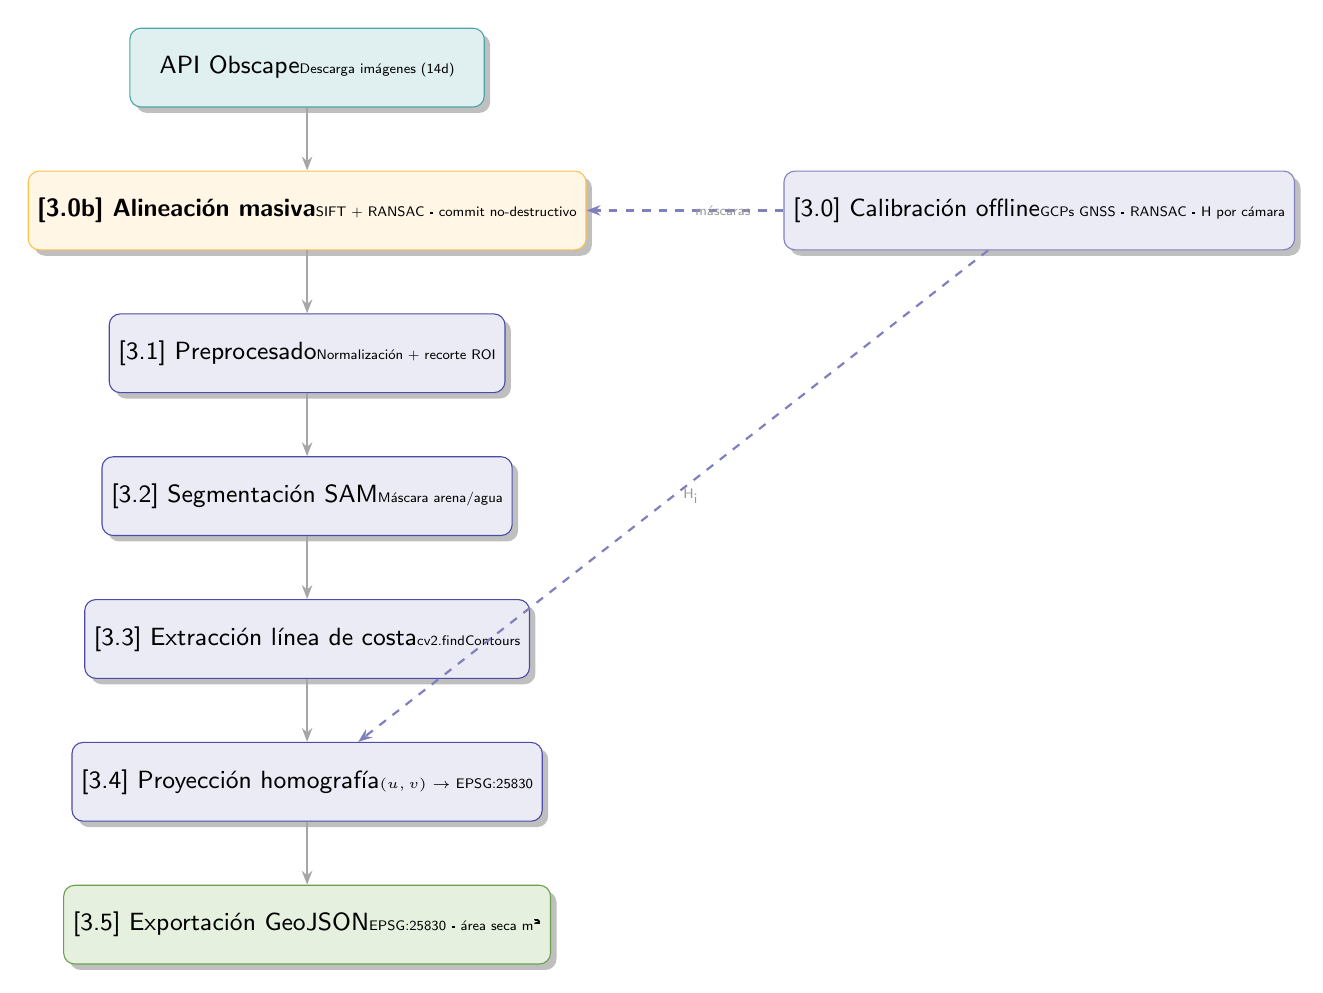
\begin{tikzpicture}[node distance=0.8cm and 1.5cm]

  % Nodos
  \node[block, fill=Teal!12, draw=Teal!70] (api)
    {API Obscape\\{\tiny Descarga imágenes (14d)}};

  \node[block, fill=Orange!10, draw=Orange!70, below=of api] (batch)
    {\textbf{[3.0b] Alineación masiva}\\{\tiny SIFT + RANSAC · commit no-destructivo}};

  \node[block, below=of batch] (preproc)
    {[3.1] Preprocesado\\{\tiny Normalización + recorte ROI}};

  \node[block, below=of preproc] (sam)
    {[3.2] Segmentación SAM\\{\tiny Máscara arena/agua}};

  \node[block, below=of sam] (extract)
    {[3.3] Extracción línea de costa\\{\tiny cv2.findContours}};

  \node[block, below=of extract] (proj)
    {[3.4] Proyección homografía\\{\tiny $(u,v) \rightarrow$ EPSG:25830}};

  \node[block, fill=OliveGreen!10, draw=OliveGreen!70, below=of proj] (export)
    {[3.5] Exportación GeoJSON\\{\tiny EPSG:25830 · área seca m²}};

  \node[block, fill=NavyBlue!8, draw=NavyBlue!50, right=2.5cm of batch] (calib)
    {[3.0] Calibración offline\\{\tiny GCPs GNSS · RANSAC · H por cámara}};

  % Flechas verticales
  \draw[arrow] (api) -- (batch);
  \draw[arrow] (batch) -- (preproc);
  \draw[arrow] (preproc) -- (sam);
  \draw[arrow] (sam) -- (extract);
  \draw[arrow] (extract) -- (proj);
  \draw[arrow] (proj) -- (export);

  % Calibración lateral
  \draw[arrow, dashed, color=NavyBlue!50] (calib) -- (proj)
    node[midway, right, label] {H\textsubscript{i}};
  \draw[arrow, dashed, color=NavyBlue!50] (calib) -- (batch)
    node[midway, right, label] {máscaras};

\end{tikzpicture}
\caption{Pipeline completo de procesamiento cv-lit}
\label{fig:pipeline}
\end{figure}

% ==============================================================
\chapter{Calibración Geométrica}
\label{ch:calibration}
% ==============================================================

\section{Fundamento matemático}

La calibración estima la \textbf{homografía planar} $\mathbf{H}$ (matriz $3\times3$) que
transforma coordenadas de imagen $(u,v)$ a coordenadas métricas $(X,Y)$ en EPSG:25830:

\begin{equation}
  \begin{pmatrix} X \\ Y \\ 1 \end{pmatrix}
  \sim
  \mathbf{H}
  \begin{pmatrix} u \\ v \\ 1 \end{pmatrix}
  \label{eq:homography}
\end{equation}

La hipótesis de planaridad es válida dado que el objeto de interés (línea de costa) es
aproximadamente plano a escala de cada cámara.

\subsection{Corrección de distorsión radial}

Antes de estimar $\mathbf{H}$, los puntos imagen se corrigen con los parámetros intrínsecos:

\begin{equation}
  \mathbf{K} = \begin{pmatrix} f_x & 0 & c_x \\ 0 & f_y & c_y \\ 0 & 0 & 1 \end{pmatrix},
  \quad
  \mathbf{D} = (k_1, k_2, p_1, p_2, k_3)
\end{equation}

Implementado via \texttt{cv2.calibrateCamera()} con tablero de ajedrez o GCPs propios.

\subsection{Estimación RANSAC}

\begin{codebox}[Estimación de homografía con RANSAC]
\begin{minted}{python}
H, mask = cv2.findHomography(
    pts_img,            # puntos imagen (u,v)
    pts_world,          # coordenadas UTM (X,Y) en EPSG:25830
    cv2.RANSAC,
    ransacReprojThreshold=5.0   # umbral de reproyección (px)
)
\end{minted}
\end{codebox}

\section{Proceso de calibración por cámara}

\begin{enumerate}[leftmargin=1.5em]
  \item \textbf{Recepción de GCPs} del IEL: puntos de control con coordenadas $(X,Y,Z)$
        en EPSG:25830 y su correspondiente píxel imagen $(u,v)$. Mínimo 4 pares; recomendado $\geq 8$.
  \item \textbf{Marcado interactivo} con \texttt{calibration\_tool.py}:
        \begin{itemize}
          \item Click izquierdo → punto de \textit{calibración} (verde)
          \item Click derecho → punto de \textit{validación} (azul, no usado en H)
          \item Tecla \texttt{h} → estimación RANSAC
          \item Tecla \texttt{s} → guardar perfil
          \item Tecla \texttt{p} → exportar imagen de diagnóstico
        \end{itemize}
  \item \textbf{Validación ciega}: el RMSE se calcula por separado sobre los puntos de
        validación (no vistos en RANSAC), garantizando una estimación honesta del error.
  \item \textbf{Guardar perfil}: \texttt{calibration/cam\_N\_profile.json} con $\mathbf{H}$,
        metadatos, RMSE calibración/validación y fecha.
\end{enumerate}

\section{Resultados de calibración (junio 2026)}

\begin{table}[H]
\centering
\caption{Resultados de precisión por cámara}
\label{tab:calibration-results}
\begin{tabular}{C{1.8cm} C{1.8cm} C{2.5cm} C{2.5cm} C{2.5cm} C{2.2cm}}
\toprule
\textbf{Cámara} & \textbf{GCPs} & \textbf{RMSE Cal. (m)} & \textbf{RMSE Val. (m)} & \textbf{RMSE Val. (px)} & \textbf{Estado} \\
\midrule
CAM~1 & 51 & 1.53 & \textbf{1.45} & 19.36 & \textcolor{OliveGreen}{OK} \\
CAM~2 & 39 & 2.64 & 3.45          & 21.09 & \textcolor{Goldenrod}{Revisar} \\
CAM~3 & 49 & 1.61 & 2.32          & 38.38 & \textcolor{OliveGreen}{OK} \\
CAM~4 & 49 & 2.78 & 3.06          & 100.01 & \textcolor{Goldenrod}{Revisar} \\
CAM~5 & 61 & 1.45 & \textbf{1.38} & 14.81 & \textcolor{OliveGreen}{OK} \\
CAM~6 & 69 & 6.14 & 4.74          & 130.62 & \textcolor{BrickRed}{Critico} \\
\bottomrule
\end{tabular}
\end{table}

\begin{warnbox}[Cámaras con error elevado]
Los errores de CAM~4 (100~px) y CAM~6 (130~px) superan ampliamente el umbral de aceptación
y sugieren una de estas causas:
\begin{itemize}
  \item Distorsión radial no corregida (requiere parámetros intrínsecos reales).
  \item Inconsistencia en los puntos manuales (GCPs marcados con baja precisión).
  \item Movimiento de la cámara entre la toma de referencia y la calibración.
\end{itemize}
\textbf{Acción recomendada:} recalibrar con \texttt{recalibrate.py --cam 4} y \texttt{--cam 6}
sobre imágenes actuales, revisando la distribución espacial de los GCPs.
\end{warnbox}

\section{Imágenes de diagnóstico}

Las imágenes de la figura~\ref{fig:diagnostics} muestran la reproyección de GCPs sobre las
imágenes de referencia. Los vectores de error se representan magnificados $\times10$.

\begin{figure}[H]
  \centering
  \begin{subfigure}[b]{0.48\textwidth}
    \includegraphics[width=\textwidth]{../calibration/diagnostics/CAM1_diagnostic.jpg}
    \caption{CAM~1 — RMSE val. 1.45~m}
  \end{subfigure}
  \hfill
  \begin{subfigure}[b]{0.48\textwidth}
    \includegraphics[width=\textwidth]{../calibration/diagnostics/CAM2_diagnostic.jpg}
    \caption{CAM~2 — RMSE val. 3.45~m}
  \end{subfigure}

  \vspace{0.4cm}
  \begin{subfigure}[b]{0.48\textwidth}
    \includegraphics[width=\textwidth]{../calibration/diagnostics/CAM3_diagnostic.jpg}
    \caption{CAM~3 — RMSE val. 2.32~m}
  \end{subfigure}
  \hfill
  \begin{subfigure}[b]{0.48\textwidth}
    \includegraphics[width=\textwidth]{../calibration/diagnostics/CAM4_diagnostic.jpg}
    \caption{CAM~4 — RMSE val. 3.06~m \textcolor{Goldenrod}{(revisar)}}
  \end{subfigure}

  \vspace{0.4cm}
  \begin{subfigure}[b]{0.48\textwidth}
    \includegraphics[width=\textwidth]{../calibration/diagnostics/CAM5_diagnostic.jpg}
    \caption{CAM~5 — RMSE val. 1.38~m}
  \end{subfigure}
  \hfill
  \begin{subfigure}[b]{0.48\textwidth}
    \includegraphics[width=\textwidth]{../calibration/diagnostics/CAM6_diagnostic.jpg}
    \caption{CAM~6 — RMSE val. 4.74~m \textcolor{BrickRed}{(crítico)}}
  \end{subfigure}

  \caption{Diagnóstico de calibración — reproyección de GCPs (vectores $\times10$)}
  \label{fig:diagnostics}
\end{figure}

\section{Recalibración rápida}

Si la cámara sufre un ligero movimiento (viento, mantenimiento), se puede actualizar la
homografía sin reintroducir coordenadas UTM:

\begin{codebox}[Recalibración]
\begin{minted}{bash}
# Arrastra los GCPs existentes sobre la imagen nueva
python3 proces_images/recalibrate.py --cam 1 --image /ruta/nueva_foto.jpg
\end{minted}
\end{codebox}

% ==============================================================
\chapter{Módulo de Alineación Masiva}
\label{ch:batch}
% ==============================================================

\section{Motivación}

El flujo anterior validaba fotogramas de forma \textbf{unitaria}: una llamada API por imagen,
sin visión global del lote. Esto presentaba tres problemas:

\begin{enumerate}[leftmargin=1.5em]
  \item \textbf{Escalabilidad}: con 24 imágenes/día por 6 cámaras, revisar manualmente cada
        alineación era inviable.
  \item \textbf{Detección de deriva}: sin comparativa global era difícil detectar si una
        cámara había girado ligeramente con el tiempo.
  \item \textbf{Objetos dinámicos}: SIFT sin restricciones detectaba gaviotas y olas como
        features, produciendo homografías sesgadas.
\end{enumerate}

\section{Arquitectura de estados}

El módulo implementa una \textbf{máquina de estados no-destructiva} de 5 fases:

\begin{figure}[H]
\centering
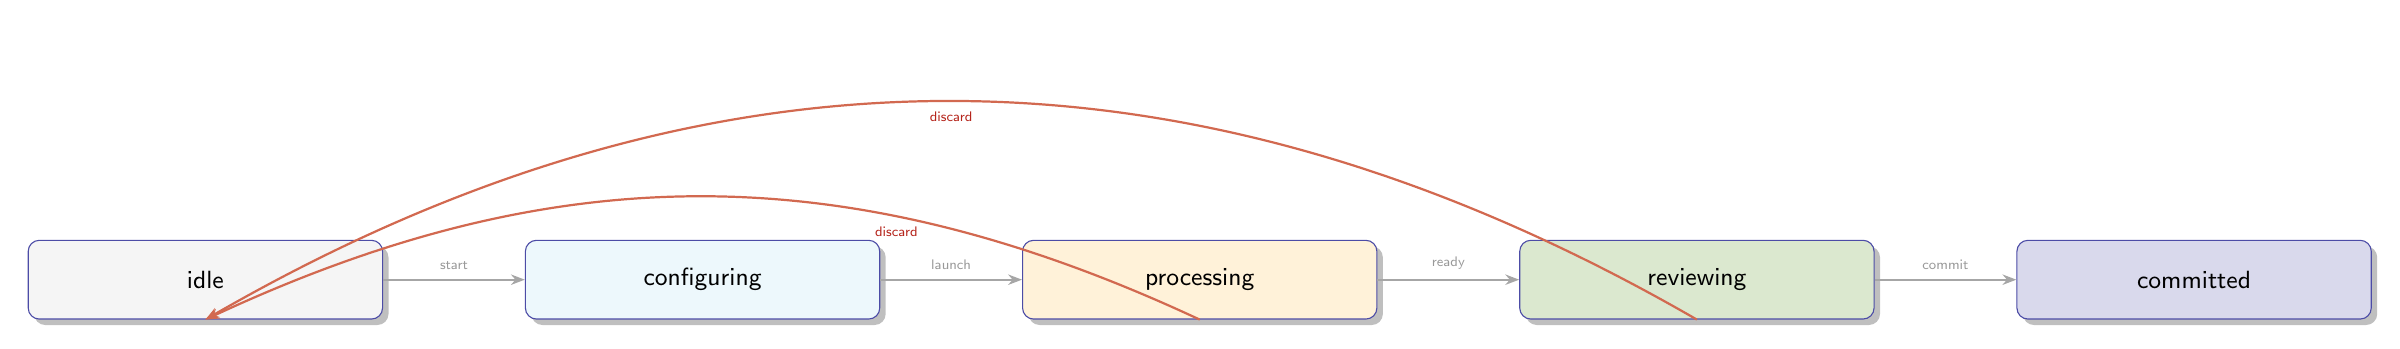
\begin{tikzpicture}[node distance=0.6cm and 1.8cm]
  \node[block, fill=gray!8] (idle) {idle};
  \node[block, fill=SkyBlue!15, right=of idle] (config) {configuring};
  \node[block, fill=Orange!15, right=of config] (proc) {processing};
  \node[block, fill=OliveGreen!15, right=of proc] (review) {reviewing};
  \node[block, fill=NavyBlue!15, right=of review] (commit) {committed};

  \draw[arrow] (idle) -- (config) node[midway,above,label]{start};
  \draw[arrow] (config) -- (proc) node[midway,above,label]{launch};
  \draw[arrow] (proc) -- (review) node[midway,above,label]{ready};
  \draw[arrow] (review) -- (commit) node[midway,above,label]{commit};

  % discard arco
  \draw[arrow, bend right=30, color=BrickRed!60]
    (review.south) to node[below,label]{\textcolor{BrickRed}{discard}} (idle.south);
  \draw[arrow, bend right=25, color=BrickRed!60]
    (proc.south) to node[below,label,pos=0.3]{\textcolor{BrickRed}{discard}} (idle.south);
\end{tikzpicture}
\caption{Máquina de estados del módulo BatchAlignment}
\label{fig:state-machine}
\end{figure}

\begin{infobox}[Principio de no-destructividad]
Todo el trabajo intermedio vive en \texttt{/tmp/cv\_lit\_batch/\{job\_id\}/}.
Los originales de cada cámara \textbf{nunca} se modifican.
La escritura permanente ocurre \textbf{únicamente} al llamar al commit explícito.
\end{infobox}

\subsection{Estructura del directorio temporal por job}

\begin{codebox}[]
\begin{minted}{text}
/tmp/cv_lit_batch/{job_id}/
  aligned/    ← imágenes con warpPerspective aplicado (staging)
  diff/       ← mapas de delta por imagen
  blend/      ← blend 50/50 en escala de grises
\end{minted}
\end{codebox}

\section{Pipeline de alineación: algoritmo}

\subsection{Parámetros configurables}

\begin{table}[H]
\centering
\caption{Parámetros del pipeline de alineación (\texttt{batch\_alignment.py})}
\label{tab:align-params}
\begin{tabular}{L{4cm} C{2.5cm} L{6cm}}
\toprule
\textbf{Constante} & \textbf{Valor} & \textbf{Descripción} \\
\midrule
\texttt{SIFT\_FEATURES}   & 3\,000 & Keypoints máximos por imagen \\
\texttt{LOWE\_RATIO}      & 0.75   & Ratio test de Lowe para filtrar matches \\
\texttt{MIN\_INLIERS}     & 15     & Inliers mínimos RANSAC (con máscara) \\
\texttt{MIN\_INLIERS\_FULL} & 30   & Inliers mínimos sin máscara (fallback) \\
\texttt{RANSAC\_THRESH}   & 5.0~px & Umbral de reproyección RANSAC \\
\bottomrule
\end{tabular}
\end{table}

\subsection{Estrategia de dos pasadas}

Para combinar la robustez de las máscaras con la resiliencia ante zonas escasas de features:

\begin{codebox}[Lógica de dos pasadas (pseudocódigo)]
\begin{minted}{python}
# Pasada 1: con máscara de zonas estables
H, inliers, n_good, fail = _try_align(gray, ref_kp, ref_des,
                                       mask=feat_mask,
                                       threshold=MIN_INLIERS)  # 15
if inliers >= MIN_INLIERS:
    result.used_mask = True
    return H, inliers

# Pasada 2 (fallback): toda la imagen, umbral más alto
H, inliers, n_good, fail = _try_align(gray, ref_kp_full, ref_des_full,
                                       mask=None,
                                       threshold=MIN_INLIERS_FULL)  # 30
result.used_mask = False
\end{minted}
\end{codebox}

\subsection{Flujo completo del pipeline}

\begin{enumerate}[leftmargin=1.5em]
  \item Carga imagen base → extrae keypoints con SIFT (con y sin máscara).
  \item Por cada imagen del lote (tarea de fondo asíncrona):
    \begin{enumerate}[leftmargin=1em]
      \item Detecta features → matching FLANN con ratio test de Lowe (0.75).
      \item RANSAC → homografía $\mathbf{H}$ (dos pasadas).
      \item \texttt{cv2.warpPerspective} → imagen alineada → \texttt{aligned/}.
      \item \texttt{\_compute\_diff\_map} → mapa de delta → \texttt{diff/}.
      \item \texttt{\_blend\_grayscale} → blend 50/50 → \texttt{blend/}.
      \item \texttt{\_compute\_mean\_shift} → métrica escalar $\delta_{\text{px}}$.
      \item Actualiza \texttt{job.progress\_current}.
    \end{enumerate}
  \item \texttt{job.status = "ready"} al finalizar.
\end{enumerate}

\section{Renderizado del mapa de delta}

El mapa de delta es una imagen compuesta de tres capas superpuestas que proporciona tanto
información visual intuitiva como métricas cuantitativas.

\subsection{Capa 1 — Heatmap de diferencia absoluta}

\begin{equation}
  \Delta_\text{abs}(i,j) = \frac{1}{3}\sum_{c \in \{R,G,B\}} |I_\text{ref}(i,j,c) - I_\text{ali}(i,j,c)|
\end{equation}

Se normaliza y se aplica \texttt{COLORMAP\_HOT} de OpenCV:

\begin{table}[H]
\centering
\caption{Leyenda del heatmap HOT}
\begin{tabular}{C{2cm} L{8cm}}
\toprule
\textbf{Color} & \textbf{Significado} \\
\midrule
Negro & $\Delta = 0$ — alineación perfecta \\
Rojo/naranja & Error de intensidad moderado \\
Amarillo & Error alto \\
Blanco & Error severo — zona mal alineada \\
\bottomrule
\end{tabular}
\end{table}

\subsection{Capa 2 — Divergencia de bordes (overlay cian)}

\begin{codebox}[]
\begin{minted}{python}
edges_ref = cv2.Canny(ref_gray, 40, 120)
edges_ali = cv2.Canny(aligned_gray, 40, 120)
edge_diff = cv2.dilate(cv2.absdiff(edges_ref, edges_ali), kernel_5x5)
composite[edge_diff > 0] = (255, 255, 0)  # cian en BGR
\end{minted}
\end{codebox}

Los bordes estructurales que \textbf{no coinciden} entre referencia y alineada aparecen en
\textbf{cian}, identificando exactamente qué objeto se desplazó y en qué dirección.

\subsection{Capa 3 — Métrica escalar $\delta_{\text{px}}$ (flujo óptico Farneback)}

\begin{equation}
  \delta_{\text{px}} = \text{mediana}\left(
    \sqrt{v_x(i,j)^2 + v_y(i,j)^2}
  \right)
\end{equation}

donde $(v_x, v_y)$ es el campo de flujo óptico residual post-warp calculado con Farneback.
Mide cuántos píxeles de desplazamiento sistemático quedan tras la homografía.

\textbf{Umbral de alerta} en la UI: $\delta_{\text{px}} > 3$.

\section{API REST del módulo}

\begin{table}[H]
\centering
\caption{Endpoints del router \texttt{/api/batch/}}
\label{tab:api-batch}
\begin{tabular}{C{1.5cm} L{5cm} L{6cm}}
\toprule
\textbf{Método} & \textbf{Ruta} & \textbf{Descripción} \\
\midrule
\texttt{POST}  & \texttt{/start}                    & Encola job + lanza pipeline en background \\
\texttt{GET}   & \texttt{/\{id\}/status}             & Polling de progreso (fase processing) \\
\texttt{GET}   & \texttt{/\{id\}/results}            & Lista completa de métricas (fase ready) \\
\texttt{GET}   & \texttt{/\{id\}/preview/original/\{fn\}} & Imagen original sin transformar \\
\texttt{GET}   & \texttt{/\{id\}/preview/aligned/\{fn\}} & Imagen alineada en staging \\
\texttt{GET}   & \texttt{/\{id\}/preview/diff/\{fn\}} & Mapa de delta compuesto \\
\texttt{GET}   & \texttt{/\{id\}/preview/blend/\{fn\}} & Blend 50/50 en escala de grises \\
\texttt{PATCH} & \texttt{/\{id\}/approve/\{fn\}}    & Override de aprobación individual \\
\texttt{POST}  & \texttt{/\{id\}/commit}             & Two-phase commit → \texttt{CAM\_X/aligned/} \\
\texttt{DELETE}& \texttt{/\{id\}}                   & Descarta job y elimina temp dir \\
\bottomrule
\end{tabular}
\end{table}

\section{Modelos de dominio}

\begin{codebox}[Dataclasses principales (batch\_alignment.py)]
\begin{minted}{python}
@dataclass
class AlignmentResult:
    filename:      str
    status:        str       # "ok" | "failed" | "reference"
    inliers:       int       # inliers RANSAC
    mean_shift_px: float     # mediana flujo óptico residual (px)
    H:             Optional[List]  # homografía 3×3 como lista plana
    approved:      bool = True     # override de aprobación por imagen
    fail_reason:   Optional[str] = None  # no_features|low_matches|ransac_failed
    used_mask:     bool = True     # True = pasada con máscara activa

@dataclass
class BatchJob:
    job_id:           str
    cam_id:           int
    base_filename:    str
    image_filenames:  List[str]
    status:           str    # pending|processing|ready|committed|failed|discarded
    results:          Dict[str, AlignmentResult]
    progress_current: int
    progress_total:   int
\end{minted}
\end{codebox}

\section{Flujo de commit (two-phase write)}

\begin{figure}[H]
\centering
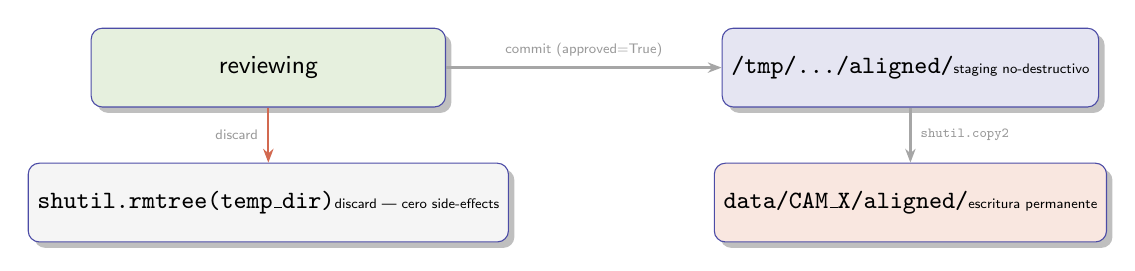
\begin{tikzpicture}[node distance=0.7cm and 2cm]
  \node[block, fill=OliveGreen!10] (review) {reviewing};
  \node[block, fill=NavyBlue!10, right=3.5cm of review] (staging)
    {\texttt{/tmp/.../aligned/}\\{\tiny staging no-destructivo}};
  \node[block, fill=BrickRed!8, below=of staging] (disk)
    {\texttt{data/CAM\_X/aligned/}\\{\tiny escritura permanente}};
  \node[block, fill=gray!8, below=of review] (discard)
    {\texttt{shutil.rmtree(temp\_dir)}\\{\tiny discard — cero side-effects}};

  \draw[arrow] (review) -- (staging) node[midway,above,label]{commit (approved=True)};
  \draw[arrow] (staging) -- (disk) node[midway,right,label]{\texttt{shutil.copy2}};
  \draw[arrow, color=BrickRed!60] (review) -- (discard) node[midway,left,label]{discard};
\end{tikzpicture}
\caption{Flujo de commit no-destructivo}
\end{figure}

% ==============================================================
\chapter{Máscaras de Zonas Estables SIFT}
\label{ch:masks}
% ==============================================================

\section{Problema: objetos dinámicos en SIFT}

Sin restricciones de zona, SIFT detecta features en \textbf{cualquier región} de la imagen,
incluyendo objetos dinámicos que producen correspondencias erróneas:

\begin{itemize}[leftmargin=1.5em]
  \item \textbf{Gaviotas y pájaros} en vuelo (zona de cielo/horizonte bajo)
  \item \textbf{Olas y espuma} de mar (bordes dinámicos muy contrastados)
  \item \textbf{Personas y bañistas} en la playa
  \item \textbf{Sombras dinámicas} de nubes
\end{itemize}

Resultado: matches entre objetos en posiciones distintas entre tomas → homografía sesgada
→ imágenes ``giradas'' o desplazadas incorrectamente.

\section{Solución: máscaras de regiones estables}

El fichero \texttt{calibration/alignment\_masks.json} define zonas con \textbf{coordenadas
fraccionarias} $(0.0 \ldots 1.0)$ independientes de la resolución real de la imagen:

\begin{equation}
  x_\text{frac} = \frac{x_\text{px}}{W_\text{imagen}}, \quad
  y_\text{frac} = \frac{y_\text{px}}{H_\text{imagen}}
\end{equation}

\begin{codebox}[alignment\_masks.json — estructura]
\begin{minted}{json}
{
  "CAM_1": {
    "regions": [
      {"label": "horizonte_mar",   "x0": 0.00, "y0": 0.31, "x1": 1.00, "y1": 0.40},
      {"label": "arena_baja",      "x0": 0.00, "y0": 0.73, "x1": 0.60, "y1": 0.88},
      {"label": "vegetacion_dcha", "x0": 0.60, "y0": 0.73, "x1": 1.00, "y1": 0.92}
    ]
  }
}
\end{minted}
\end{codebox}

\section{Zonas por cámara}

\begin{table}[H]
\centering
\caption{Configuración de máscaras SIFT por cámara}
\label{tab:masks}
\begin{tabular}{C{1.5cm} L{3.5cm} C{3.5cm} L{4.5cm}}
\toprule
\textbf{Cámara} & \textbf{Zona 1} & \textbf{Zona 2} & \textbf{Justificación} \\
\midrule
CAM~1 & Horizonte mar (y=0.31--0.40) & Arena baja + Vegetación dcha & Excluye cielo con gaviotas \\
CAM~2 & Horizonte (y=0.26--0.40)    & El Peñón (x=0.58--0.88)     & El Peñón de Ifach es referencia fija excelente \\
CAM~3 & Horizonte (y=0.34--0.48)    & Edificio dcha (x=0.72--1.00) & Edificio como anclaje vertical \\
CAM~4 & Horizonte (y=0.30--0.44)    & Edificio izq (x=0.00--0.28)  & Edificio como anclaje vertical \\
CAM~5 & Horizonte (y=0.28--0.42)    & Zona izq (x=0.00--0.32)      & \\
CAM~6 & Horizonte (y=0.32--0.46)    & Edificios izq (x=0.00--0.35) & \\
\bottomrule
\end{tabular}
\end{table}

\section{Corrección CAM\_1: problema de gaviotas}

\begin{figure}[H]
  \centering
  \begin{subfigure}[b]{0.48\textwidth}
    \includegraphics[width=\textwidth]{img_cam1_mask_actual.jpg}
    \caption{Máscara anterior — zona ``horizonte'' comienza en $y=0{,}24$, alcanzando el cielo con gaviotas}
  \end{subfigure}
  \hfill
  \begin{subfigure}[b]{0.48\textwidth}
    \includegraphics[width=\textwidth]{img_cam1_mask_propuesta.jpg}
    \caption{Máscara corregida — \texttt{horizonte\_mar} comienza en $y=0{,}31$ (mar), más arena baja y vegetación}
  \end{subfigure}
  \caption{Comparativa de máscaras SIFT para CAM~1 (imagen 4608$\times$2682~px)}
  \label{fig:mask-cam1}
\end{figure}

\begin{infobox}[Por qué CAM\_1 es problemática]
La cámara apunta hacia el norte sobre la playa. En imágenes de mañana, 5--10 gaviotas
sobrevuelan habitualmente en la banda $y \approx 0{,}14 \ldots 0{,}30$ (cielo bajo).

SIFT detecta las aves como features de alto contraste con gran confianza. Al estar en
posiciones distintas entre tomas, generan matches cruzados que sesgan la homografía.

La corrección: \texttt{horizonte\_mar} ($y=0{,}31 \ldots 0{,}40$) está en la franja de agua
cerca del horizonte, donde los features son reproducibles y estables.
\end{infobox}

\subsection{Coordenadas en píxeles (imagen 4608$\times$2682)}

\begin{table}[H]
\centering
\caption{Conversión fracción → píxeles para CAM\_1}
\begin{tabular}{L{4cm} C{4cm} C{4cm}}
\toprule
\textbf{Zona} & \textbf{Esquina sup-izq (px)} & \textbf{Esquina inf-der (px)} \\
\midrule
\texttt{horizonte\_mar}   & (0,~831)    & (4608,~1072) \\
\texttt{arena\_baja}      & (0,~1957)   & (2764,~2360) \\
\texttt{vegetacion\_dcha} & (2764,~1957)& (4608,~2467) \\
\bottomrule
\end{tabular}
\end{table}

\section{Cómo ajustar una máscara}

\begin{enumerate}[leftmargin=1.5em]
  \item Abrir una imagen real de la cámara en un visor que muestre coordenadas de píxel.
  \item Identificar las regiones estables (sin gaviotas, olas ni personas).
  \item Anotar las coordenadas en píxeles de las esquinas.
  \item Convertir a fracciones: $x_f = x_\text{px}/W$, $y_f = y_\text{px}/H$.
  \item Editar \texttt{calibration/alignment\_masks.json}.
  \item Ejecutar el script de verificación:
\end{enumerate}

\begin{codebox}[Script de verificación visual de máscaras]
\begin{minted}{python}
import cv2, json, numpy as np

IMG   = "proces_images/data/camera1/IMAGEN_REF.jpg"
MASKS = "calibration/alignment_masks.json"
CAM   = "CAM_1"

img = cv2.imread(IMG)
h, w = img.shape[:2]
overlay = img.copy()

with open(MASKS) as f:
    cfg = json.load(f)

for r in cfg[CAM]["regions"]:
    x0, y0 = int(r["x0"]*w), int(r["y0"]*h)
    x1, y1 = int(r["x1"]*w), int(r["y1"]*h)
    cv2.rectangle(overlay, (x0,y0), (x1,y1), (0,255,0), -1)
    cv2.putText(overlay, r["label"], (x0+10, y0+30),
                cv2.FONT_HERSHEY_SIMPLEX, 0.8, (0,0,0), 2)

result = cv2.addWeighted(img, 0.5, overlay, 0.5, 0)
cv2.imwrite("/tmp/mask_check.jpg", result)
print(f"Guardado en /tmp/mask_check.jpg  ({w}x{h})")
\end{minted}
\end{codebox}

% ==============================================================
\chapter{Interfaz Web}
\label{ch:frontend}
% ==============================================================

\section{Arquitectura frontend}

La interfaz web está construida con \textbf{Vue 3} + \textbf{Vite} + \textbf{Tailwind CSS},
sin gestión de estado global (no Pinia): cada componente mantiene su propio estado reactivo
con \texttt{ref()} y \texttt{reactive()}.

Para iniciar el entorno de desarrollo:

\begin{codebox}[]
\begin{minted}{bash}
./start_dev.sh
# Backend:  http://localhost:8000
# Frontend: http://localhost:5173
\end{minted}
\end{codebox}

\section{Componente BatchAlignment.vue}

Componente principal del módulo de alineación masiva. Integrado en el \textbf{paso 3}
del flujo de calibración (\texttt{Calibration.vue}).

\subsection{Variables de estado}

\begin{codebox}[]
\begin{minted}{javascript}
const phase    = ref('idle')   // idle|configuring|processing|reviewing|committed
const jobId    = ref(null)     // UUID del job backend activo
const results  = ref([])       // Array de AlignmentResult del lote
const selected = ref(null)     // filename seleccionado en filmstrip
const viewMode = ref('diff')   // 'diff' | 'blend' | 'aligned'
\end{minted}
\end{codebox}

\subsection{Props y eventos}

\begin{table}[H]
\centering
\caption{Props del componente BatchAlignment}
\begin{tabular}{L{3cm} L{2.5cm} L{7cm}}
\toprule
\textbf{Prop} & \textbf{Tipo} & \textbf{Descripción} \\
\midrule
\texttt{camId}       & Number & ID de cámara (1--6) \\
\texttt{imageList}   & Array  & Lista de imágenes disponibles \\
\texttt{initialBase} & String & Imagen base por defecto (del perfil de calibración) \\
\midrule
\textbf{Emit} & \textbf{Payload} & \textbf{Descripción} \\
\midrule
\texttt{notify}    & (msg, type) & Toast del sistema \\
\texttt{committed} & \{jobId, committed\} & Lote confirmado con éxito \\
\texttt{discard}   & — & Usuario descartó el job \\
\bottomrule
\end{tabular}
\end{table}

\subsection{Layout de la fase reviewing}

\begin{codebox}[Vista de revisión — esquema]
\begin{minted}{text}
+----------------------+--------------------------------------------------+
| RESUMEN              | [Mapa delta]  [Blend 50/50]  [Alineada]          |
|  Aprobadas: 44       +----------------------+---------------------------+
|  Omitidas:   3       |                      |                           |
|  Fallidas:   0       |     ORIGINAL         |    DELTA / BLEND / ALI    |
+----------------------|     <img>            |    <img>                  |
| FILMSTRIP            |                      |                           |
| ● img_001  OK        +----------------------+---------------------------+
| ▶ img_002  ~2.1px    |  Leyenda: ■negro=OK ■rojo=error ■cian=bordes    |
| ● img_003  FAIL      |                                                   |
| ● img_004  SKIP      |  inliers: 152  delta: 1.4 px  [✓ Aprobada]      |
|   ...                |                                                   |
+----------------------+--------------------------------------------------+
|  [Confirmar lote (44)]                    [Descartar sin guardar]        |
+-------------------------------------------------------------------------+
\end{minted}
\end{codebox}

\subsection{Indicadores del filmstrip}

\begin{table}[H]
\centering
\caption{Código de color en el filmstrip}
\begin{tabular}{C{2.5cm} L{4cm} L{6cm}}
\toprule
\textbf{Color} & \textbf{Estado} & \textbf{Condición} \\
\midrule
\cellcolor{NavyBlue!30} Azul   & Referencia  & Imagen base seleccionada \\
\cellcolor{OliveGreen!30} Verde & OK          & $\delta_\text{px} \leq 3$ \\
\cellcolor{Goldenrod!50} Amarillo & Drift     & $\delta_\text{px} > 3$ \\
\cellcolor{Orange!40} Ámbar   & Desaprobada & \texttt{approved = false} (manual) \\
\cellcolor{BrickRed!30} Rojo   & Fallida     & RANSAC insuficiente \\
\bottomrule
\end{tabular}
\end{table}

\subsection{Polling de progreso}

El frontend consulta el estado del job cada \textbf{800~ms} durante la fase de procesamiento:

\begin{codebox}[]
\begin{minted}{javascript}
function _poll() {
  // GET /api/batch/{jobId}/status
  if (data.status === 'ready') {
    clearInterval(pollTimer)
    await _loadResults()   // carga métricas completas
    phase.value = 'reviewing'
  }
  if (data.status === 'failed') {
    clearInterval(pollTimer)
    emit('notify', data.error, 'error')
    phase.value = 'configuring'
  }
  progress.value = data.progress_current / data.progress_total
}
\end{minted}
\end{codebox}

\section{Flujo completo de uso}

\begin{enumerate}[leftmargin=1.5em, label=\textbf{\arabic*.}]
  \item Dashboard → seleccionar cámara → pestaña \textit{Calibración} → paso 3.
  \item Elegir imagen base de referencia del lote.
  \item Pulsar ``Alinear lote completo'' → barra de progreso en tiempo real.
  \item Revisar filmstrip: verde = OK, rojo = error.
  \item Para cada imagen roja o amarilla: inspeccionar mapa de delta / blend.
  \item Desaprobar imágenes concretas (opcional) con toggle en el visor.
  \item Pulsar ``Confirmar lote'' → imágenes aprobadas a \texttt{data/CAM\_X/aligned/}.
  \item Las imágenes originales en \texttt{data/CAM\_X/images/} quedan \textbf{intactas}.
\end{enumerate}

% ==============================================================
\chapter{Región de Interés (ROI)}
\label{ch:roi}
% ==============================================================

\section{Criterios de delimitación}

Para optimizar la segmentación con SAM y reducir ruido en la extracción de línea de costa,
cada cámara tiene una ROI que excluye:

\begin{itemize}[leftmargin=1.5em]
  \item \textbf{Cielo}: píxeles por encima del horizonte.
  \item \textbf{Infraestructura}: paseos marítimos, espigones, edificios fuera de la zona de interés.
  \item \textbf{Mar profundo}: zona sin rotura de onda donde la línea de costa no es visible.
\end{itemize}

\section{Coordenadas por cámara}

Las ROIs se almacenan en \texttt{calibration/roi\_config.json}:

\begin{table}[H]
\centering
\caption{ROIs preliminares por cámara (a ajustar con imágenes de producción)}
\label{tab:roi}
\begin{tabular}{C{2cm} C{4.5cm} L{6cm}}
\toprule
\textbf{Cámara} & \textbf{ROI $(x_0, y_0, x_1, y_1)$ px} & \textbf{Justificación} \\
\midrule
CAM~1 & [0, 400, 1920, 1080]  & Recorte superior (horizonte $\approx y=400$) \\
CAM~2 & [0, 350, 1920, 1080]  & Horizonte más bajo \\
CAM~3 & [0, 450, 1920, 1080]  & Ángulo con más cielo visible \\
CAM~4 & [0, 400, 1920, 1080]  & \\
CAM~5 & [0, 380, 1920, 1080]  & \\
CAM~6 & [0, 420, 1920, 1080]  & \\
\bottomrule
\end{tabular}
\end{table}

\begin{warnbox}[Nota de actualización]
Estos valores son preliminares y se ajustarán tras la primera recepción de imágenes de
producción de todas las cámaras de Guardamar. Verificar superposición ROI sobre imagen
real para confirmar que no se pierde zona de intermarea.
\end{warnbox}

% ==============================================================
\chapter{Segmentación y Extracción de Línea de Costa}
\label{ch:segmentation}
% ==============================================================

\section{Segmentación semántica con SAM}

Se utiliza \textbf{Segment Anything Model (SAM)} de Meta AI en modo \textit{zero-shot}:
sin datos de entrenamiento específicos de Guardamar.

\begin{itemize}[leftmargin=1.5em]
  \item \textbf{Modo de uso}: prompt basado en puntos semilla o bounding boxes de la ROI.
  \item \textbf{Salida}: mapa probabilístico arena seca / arena húmeda / agua.
  \item \textbf{Post-SAM}: umbral adaptativo + filtrado morfológico → máscara binaria.
\end{itemize}

\begin{codebox}[Segmentación (extracto segmentation\_sam.py)]
\begin{minted}{python}
from segment_anything import sam_model_registry, SamAutomaticMaskGenerator

sam = sam_model_registry["vit_h"](checkpoint=SAM_CHECKPOINT)
mask_generator = SamAutomaticMaskGenerator(
    sam,
    points_per_side=32,
    pred_iou_thresh=0.86,
    stability_score_thresh=0.92
)
masks = mask_generator.generate(roi_img)
\end{minted}
\end{codebox}

\section{Extracción de línea de costa}

\begin{enumerate}[leftmargin=1.5em]
  \item Cálculo de contornos sobre la máscara binaria:
        \texttt{cv2.findContours(mask, cv2.RETR\_EXTERNAL, cv2.CHAIN\_APPROX\_SIMPLE)}
  \item Selección del contorno correspondiente al borde arena húmeda -- arena seca.
  \item Resultado: polilínea en coordenadas píxel $(u, v)$.
\end{enumerate}

\section{Proyección a EPSG:25830}

Aplicación de la homografía~\eqref{eq:homography} para transformar cada punto $(u,v)$
de la polilínea a coordenadas métricas:

\begin{codebox}[]
\begin{minted}{python}
def pixel_to_utm(H, pts_px):
    """pts_px: Nx2 array de (u,v). Retorna Nx2 en UTM EPSG:25830."""
    pts_h = np.hstack([pts_px, np.ones((len(pts_px), 1))])
    result = (H @ pts_h.T).T
    return result[:, :2] / result[:, 2:3]   # normalización homogénea
\end{minted}
\end{codebox}

\section{Exportación GeoJSON}

\begin{codebox}[Estructura del GeoJSON de salida]
\begin{minted}{json}
{
  "type": "FeatureCollection",
  "crs": {
    "type": "name",
    "properties": { "name": "EPSG:25830" }
  },
  "features": [{
    "type": "Feature",
    "geometry": {
      "type": "LineString",
      "coordinates": [[711234.5, 4209876.3], ["..."]]
    },
    "properties": {
      "ID_Camara":     1,
      "Timestamp":     "2026-04-30T12:00:00Z",
      "Confianza_IA":  0.93,
      "Area_Seca_m2":  14250.7
    }
  }]
}
\end{minted}
\end{codebox}

% ==============================================================
\chapter{Validación y Métricas de Calidad}
\label{ch:validation}
% ==============================================================

\section{Estrategia de validación}

Comparación de la línea detectada contra \textbf{transectos GNSS independientes} del IEL:
puntos \textbf{no usados} en la calibración de homografía.

\section{Métricas}

\begin{equation}
  \text{RMSE} = \sqrt{\frac{1}{N} \sum_{i=1}^{N} d_i^2}
  \qquad
  \text{MAE} = \frac{1}{N} \sum_{i=1}^{N} d_i
\end{equation}

donde $d_i$ es la distancia mínima en metros del punto GNSS $i$ a la polilínea detectada.

\section{Criterios de aceptación}

\begin{table}[H]
\centering
\caption{Umbrales de calidad del sistema}
\begin{tabular}{L{4cm} C{3cm} L{5.5cm}}
\toprule
\textbf{Métrica} & \textbf{Objetivo} & \textbf{Condición} \\
\midrule
RMSE geométrico    & $< 1{,}5$~m & Condiciones estándar (12:00h, sin interferencias) \\
MAE geométrico     & $< 1{,}0$~m & Objetivo secundario \\
Cobertura temporal & $\geq 90\%$ & Imágenes a 12:00h procesadas sin error \\
$\delta_\text{px}$ alineación & $< 3$~px & Drift residual post-homografía \\
\bottomrule
\end{tabular}
\end{table}

\section{Factores de error a monitorizar}

\begin{itemize}[leftmargin=1.5em]
  \item \textbf{Calidad de imagen}: niebla, reflejo solar, lluvia, espuma excesiva.
  \item \textbf{Nivel de marea}: afecta la posición real de la línea (calibrar en diferentes estados de marea).
  \item \textbf{Deriva de cámara}: movimiento del soporte por viento, mantenimiento u otras causas.
  \item \textbf{Precisión GCPs}: exactitud del levantamiento GNSS del IEL (instrumental + propagación de error).
\end{itemize}

\section{Validación en QGIS}

\begin{enumerate}[leftmargin=1.5em]
  \item Configurar CRS del proyecto en \textbf{EPSG:25830}.
  \item Cargar GCPs del IEL como capa de puntos.
  \item Arrastrar los GeoJSON de \texttt{data/processed/lines/} al proyecto.
  \item Usar ``Distancia a la polilínea más cercana'' para calcular $d_i$.
  \item Comparar con ortofoto PNOA (WMS/WMTS del IGN) para validación visual.
\end{enumerate}

% ==============================================================
\chapter{Estado del Proyecto y Roadmap}
\label{ch:roadmap}
% ==============================================================

\section{Estado actual (junio 2026)}

\begin{table}[H]
\centering
\caption{Estado de hitos del proyecto}
\label{tab:roadmap}
\begin{tabular}{C{1cm} L{5cm} C{1.5cm} L{5cm}}
\toprule
\textbf{Mes} & \textbf{Objetivo} & \textbf{Estado} & \textbf{Nota} \\
\midrule
1 & Preparación datos + diseño interfaces & \textcolor{OliveGreen}{Hecho} & Completado \\
2 & Calibración geométrica                & \textcolor{OliveGreen}{Hecho} & 6 perfiles generados \\
3 & Segmentación (prototipo)              & \textcolor{OliveGreen}{Hecho} & SAM funcional \\
4 & Extracción línea + georreferenciación & \textcolor{OliveGreen}{Hecho} & GeoJSON en EPSG:25830 \\
5 & Validación y robustez                 & \textcolor{Goldenrod}{Parcial} & CAM 4 y 6 pendientes \\
6 & Integración y entrega                 & \textcolor{gray}{Pendiente}   & Próximo hito \\
\bottomrule
\end{tabular}
\end{table}

\section{Completado en la iteración de junio 2026}

\begin{itemize}[leftmargin=1.5em]
  \item[$\bullet$] Módulo de alineación masiva no-destructiva (\texttt{batch\_alignment.py})
    \begin{itemize}
      \item Router FastAPI \texttt{/api/batch/} con 10 endpoints
      \item Pipeline async SIFT+FLANN+RANSAC sobre lote completo
      \item Mapa de delta compuesto (heatmap HOT + edge-diff cian + métrica Farneback)
      \item Two-phase commit: staging \texttt{/tmp/} → escritura permanente sólo en commit
    \end{itemize}
  \item[$\bullet$] Interfaz de validación por lotes (\texttt{BatchAlignment.vue})
  \item[$\bullet$] Corrección de máscaras SIFT para CAM~1 (problema de gaviotas)
  \item[$\bullet$] Integración en paso 3 del flujo de calibración (\texttt{Calibration.vue})
  \item[$\bullet$] Documentación completa (esta memoria)
\end{itemize}

\section{Fase 3 — Automatización y robustez (mes 5)}

\begin{enumerate}[leftmargin=1.5em]
  \item \textbf{Procesamiento por lotes}: integrar backend para procesar todas las imágenes de 12:00h.
  \item \textbf{Filtros de calidad}: rechazo automático de imágenes con niebla o baja confianza de SAM.
  \item \textbf{Persistencia GeoJSON}: guardar histórico de líneas de costa en base de datos/sistema de ficheros.
  \item \textbf{Recalibración CAM~4 y CAM~6}: reducir RMSE por debajo de 1.5~m.
\end{enumerate}

\section{Fase 4 — Entrega e integración (mes 6)}

\begin{enumerate}[leftmargin=1.5em]
  \item Dashboard de histórico: gráficas de evolución del área seca.
  \item Exportación masiva: informes mensuales de variación de línea de costa.
  \item Manual de usuario: documentación final para el personal del Ayuntamiento.
\end{enumerate}

% ==============================================================
\chapter{Guía de Operación}
\label{ch:ops}
% ==============================================================

\section{Inicio rápido}

\begin{codebox}[Arrancar el sistema completo]
\begin{minted}{bash}
# 1. Activar entorno Conda
conda activate cv-lit

# 2. Iniciar backend + frontend en paralelo
./start_dev.sh
# Backend:  http://localhost:8000 (FastAPI + docs en /docs)
# Frontend: http://localhost:5173 (Vue 3 + Vite)
\end{minted}
\end{codebox}

\section{Descarga de imágenes}

\begin{codebox}[]
\begin{minted}{bash}
# Descarga estándar (últimas 2 semanas, 12:00h)
python3 acces_api/scheduled_download.py

# Diagnóstico de estado de cámaras
python3 scripts/verify_setup.py
\end{minted}
\end{codebox}

\section{Calibración}

\begin{codebox}[]
\begin{minted}{bash}
# Herramienta completa de calibración
python3 proces_images/calibration_tool.py --cam 1 --image /ruta/foto.jpg

# Lanzador visual rápido (CAM 1, imagen más reciente)
python3 scripts/visualizar_calibracion.py

# Recalibración rápida (cámara movida levemente)
python3 proces_images/recalibrate.py --cam 1 --image /ruta/nueva_foto.jpg

# Verificar motor matemático
python3 proces_images/test_calibration_logic.py
\end{minted}
\end{codebox}

\section{Alineación masiva (CLI)}

Para usar el módulo de alineación sin interfaz web:

\begin{codebox}[]
\begin{minted}{bash}
# Alinear todas las imágenes de una carpeta respecto a la primera
python3 homography/align_images.py \
  --input  /ruta/imagenes/ \
  --output /ruta/salida/ \
  --cam 1                    # aplica máscaras SIFT de CAM_1

# Especificar imagen de referencia manualmente
python3 homography/align_images.py \
  --input  /ruta/imagenes/ \
  --output /ruta/salida/ \
  --ref    imagen_base.jpg \
  --cam 2
\end{minted}
\end{codebox}

Salidas:
\begin{itemize}[leftmargin=1.5em]
  \item \texttt{/output/aligned/} — imágenes alineadas
  \item \texttt{/output/diagnostics/} — visualizaciones de matches
  \item \texttt{/output/homographies.csv} — métricas y matrices $H$ por imagen
\end{itemize}

\section{Pipeline de extracción}

\begin{codebox}[]
\begin{minted}{bash}
# Prototipo completo: ROI → Segmentación SAM → Línea de costa
python3 proces_images/test_mes3_pipeline.py --cam 1
\end{minted}
\end{codebox}

% ==============================================================
\chapter{Instalación y Configuración}
\label{ch:setup}
% ==============================================================

\section{Requisitos del sistema}

\begin{table}[H]
\centering
\caption{Requisitos hardware y software}
\begin{tabular}{L{4cm} L{8cm}}
\toprule
\textbf{Componente} & \textbf{Requisito mínimo} \\
\midrule
SO & Linux (Ubuntu 22.04+) o Windows 10+ \\
Python & 3.11+ \\
RAM & 8 GB (16 GB recomendado para SAM) \\
GPU & CUDA opcional pero recomendada para SAM \\
Almacenamiento & 50 GB para datos (6 cámaras × 24h/día) \\
Node.js & 18+ (para frontend) \\
\bottomrule
\end{tabular}
\end{table}

\section{Instalación del entorno Python}

\begin{codebox}[]
\begin{minted}{bash}
conda create -n cv-lit python=3.11
conda activate cv-lit

# Visión + álgebra
pip install opencv-python numpy scipy pandas

# Backend API
pip install fastapi uvicorn python-multipart

# Segmentación SAM
pip install torch torchvision
pip install git+https://github.com/facebookresearch/segment-anything.git

# Geo
pip install gdal pyproj shapely
\end{minted}
\end{codebox}

\section{Instalación del frontend}

\begin{codebox}[]
\begin{minted}{bash}
cd frontend
npm install
npm run dev       # modo desarrollo
npm run build     # build de producción (dist/)
\end{minted}
\end{codebox}

\section{Configuración de la API Obscape}

Las credenciales de acceso a la API se configuran en \texttt{acces\_api/obscape\_api.py}:

\begin{table}[H]
\centering
\caption{Parámetros de conexión Obscape}
\begin{tabular}{L{4cm} L{8cm}}
\toprule
\textbf{Parámetro} & \textbf{Valor} \\
\midrule
Base URL   & \texttt{https://obscape.com/portal/api/v3/api} \\
Username   & \texttt{fuster} \\
Portal     & \texttt{https://obscape.com/portal} \\
\bottomrule
\end{tabular}
\end{table}

% ==============================================================
\appendix
% ==============================================================

\chapter{Convenciones de código y Git}
\label{app:conventions}

\section{Estrategia de ramas}

\begin{itemize}[leftmargin=1.5em]
  \item \textbf{main}: código estable y validado.
  \item \textbf{feature/nombre-modulo}: nuevas funcionalidades.
  \item \textbf{fix/descripcion-error}: correcciones.
  \item \textbf{docs/nombre-doc}: documentación.
\end{itemize}

Todo cambio debe pasar por Pull Request antes de integrar en \texttt{main}.

\section{Nomenclatura de ficheros}

Las imágenes descargadas usan el formato determinista:
\begin{center}
\texttt{UNIX\_YYYYMMDD\_HHMMSS\_REFERENCIA.jpg}
\end{center}

\section{Proyección obligatoria}

\textbf{Toda coordenada geográfica en el sistema debe estar en EPSG:25830.}
Nunca almacenar en WGS84 (EPSG:4326) salvo para visualización en APIs de mapas.

% ==============================================================
\chapter{Glosario}
\label{app:glossary}
% ==============================================================

\begin{description}[leftmargin=3cm, style=nextline]
  \item[EPSG:25830] ETRS89 / UTM zona 30N. Sistema de referencia cartográfico oficial para la Península Ibérica.
  \item[GCP] \textit{Ground Control Point}. Punto de control terrestre con coordenadas conocidas.
  \item[Homografía] Transformación proyectiva planar entre dos planos (imagen y terreno).
  \item[IEL] Instituto de Ecología Litoral. Suministra los GCPs GNSS del proyecto.
  \item[RANSAC] \textit{Random Sample Consensus}. Estimador robusto de parámetros geométricos.
  \item[ROI] \textit{Region of Interest}. Zona de la imagen relevante para el análisis.
  \item[SAM] \textit{Segment Anything Model}. Modelo de segmentación de Meta AI.
  \item[SIFT] \textit{Scale-Invariant Feature Transform}. Detector de puntos de interés invariante a escala y rotación.
  \item[RMSE] \textit{Root Mean Square Error}. Error cuadrático medio.
  \item[MAE] \textit{Mean Absolute Error}. Error medio absoluto.
  \item[Farneback] Algoritmo de flujo óptico denso para estimar campo de desplazamiento entre dos imágenes.
  \item[Inliers] Correspondencias que se ajustan al modelo estimado por RANSAC.
  \item[Two-phase commit] Patrón de escritura en dos fases: staging temporal → confirmación permanente.
  \item[Drift] Desplazamiento residual de píxeles tras la corrección de homografía.
\end{description}

% ==============================================================
\chapter{Historial de cambios}
\label{app:changelog}
% ==============================================================

\begin{table}[H]
\centering
\caption{Historial de versiones del sistema}
\begin{tabular}{C{2.5cm} L{4cm} L{7cm}}
\toprule
\textbf{Fecha} & \textbf{Componente} & \textbf{Cambio} \\
\midrule
Ene 2026 & API client & Cliente Obscape + descarga con deduplicación \\
Feb 2026 & Calibración & \texttt{calibration\_tool.py}: intrínsecos + validación ciega \\
Mar 2026 & Calibración & \texttt{recalibrate.py}: recalibración por arrastre de GCPs \\
Abr 2026 & Segmentación & Prototipo SAM + extracción de línea de costa \\
May 2026 & Georreferenciación & Proyección a EPSG:25830 + exportación GeoJSON \\
May 2026 & Calibración & Ejecución real con GCPs del IEL (6 cámaras) \\
Jun 2026 & Backend & \texttt{batch\_alignment.py}: pipeline asíncrono + 10 endpoints \\
Jun 2026 & Frontend & \texttt{BatchAlignment.vue}: máquina de estados 5 fases \\
Jun 2026 & Máscaras SIFT & \texttt{alignment\_masks.json}: zonas estables por cámara \\
Jun 2026 & CAM~1 & Corrección máscara: excluir cielo con gaviotas (y=0.24→0.31) \\
Jun 2026 & Documentación & Esta memoria técnica en \LaTeX{} \\
\bottomrule
\end{tabular}
\end{table}

%% ============================================================
\end{document}
%% ============================================================
